\documentclass[11pt,a4paper,article,oneside]{memoir}
\usepackage{tikz}
\usepackage[T1]{fontenc}
\usepackage{lmodern}
\usepackage[swedish]{babel}
\usepackage[utf8]{inputenc}
\usepackage{clrscode}
\usepackage{microtype}
\setlength{\parskip}{6pt}
\setlength{\parindent}{0pt}
\usepackage{tabularx}
%\usepackage{minibox}
\usepackage{listings}

%\usepackage[margin=1in]{geometry}



\author{Tim Olsson}

\title{Mästarprov 1}

\checkandfixthelayout{}
\begin{document}


%\begin{titlingpage}
\maketitle
%\end{titlingpage}

\newpage

\subsection{Hantverkare}

Den giriga algoritm som används går ut på att bland alla hantverkare som är kvar, låta 
hantverkaren som kräver minst antal timmar arbeta. Detta leder till en minimalkostnad 
då man minimerar väntetidskostnaderna. För att lösa problemet på ett effektivt sätt väljer vi att 
först och främst sortera listan med hantverkare, i växande ordning enligt hur många timmar 
de kräver. Därefter är det bara att iterera genom listan och addera nuvarande totalsumman med 
varje element i listan multiplicerat med 100 och hur många hantverkare som är kvar(vi betalar ju 
även för väntetid).

\begin{codebox}
    \Procname{$\proc{Hantverkare} (H[t_1..t_n]) $ }
\zi $m \gets 0$
\zi sortera $H[t_1..t_n]$ med merge sort
\zi \For $i \gets 1$ \To $\id{length} [H] $
\zi    \Do  $\id{m}  \gets \id{m} + H[i]*100*(i- \id{length} [H]+1) $
\End
\zi \Return $m$

\end{codebox}

Sorteringen av hantverkarlistan med mergesort tar $O(n log n)$. Att iterera genom listan och utföra
en konstant operation går på $O(n)$. Den totala tidskomplexiteten blir därför O(n log n);

Att algoritmen returnerar korrekt värde är nog inget konstigt 
men för att försöka visa det på ett lite mer övertygande sätt kan man tänka sig följande: 

$H[t_1..t_n]$ = sorterad lista med hantverkare efter krävda timmar.

Då n = 0, returnerar algoritmen 0. \newline
Då n = 1, returnerar algoritmen $t_1$ \newline
Då n = 2, $t_1 < t_2$ har algoritmen enbart ett fall att välja.

$t_1$ arbetar först = $100t_1*2 + 100t_2*1$ 

Hade ordningen vart annorlunda hade resultatet istället blivit: 

$t_2$ arbetar först = $100t_2*2 + 100t_1*1$ 

Eftersom $t_1 < t_2$ efter sortering får vi den minimala kostnaden genom att låta $t_1$ arbeta först.
På liknande sätt kan man resonera kringa alla n, man måste alltid multiplicera en hantverkare med n, en med n-1 osv.
Minimala kostnaden blir då att multiplicera min av hantverkarna med n, min-1 med n-1.. osv då n >= 1 och
hantverkare >= 1.
\newpage

\subsection{Höravstånd}

Ett sätt att modellera problemet på är att man föreställer sig en graf där X-axeln står för personerna och Y-axeln för
distans från personen ytterst till vänster. 

\begin{center}
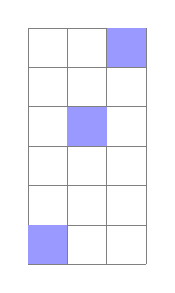
\begin{tikzpicture}
\draw[step=0.5cm,gray,very thin] (0, 0) grid (1.5,3);
\fill[blue!40!white] (0,0) rectangle (0.5,0.5);
\fill[blue!40!white] (1,1.5) rectangle (0.5,2);
\fill[blue!40!white] (1,2.5) rectangle (1.5,3); 
\end{tikzpicture}

Ex: grafen motsvarar indata P[0,3,5].
\end{center}

Problemet går ut på att få alla par av personer $(p_i, p_i+1) < k$ distans. 
Det kan i graf-formen representeras genom att man drar en linje med lutning k från varje person i grafen. Nästkommande person(er) måste då vara under linjerna för att de ska vara inom k avstånd från varandra.
Låt $L = k-1$, om vi nu drar linjer med lutning L från varje person, måste nästkommande person vara antingen på eller under linjen
((p1,p2) <= k-1 = L).
För att lösa problemet i graf-form måste vi justera vissa personers position så att ingen person ligger över linjen L, tillhörande 
personerna till dess vänster. Låt vektorn res stå för grafens residualpunkter, dvs $(x, y-Lx)$ för varje $(x,y)$. Problemet 
kan då formuleras så att man ska få residualvektorn att vara icke-växande på minsta antal förflyttningar(Att byta siffra på ett tal i res motsvarar en förflyttning i storlek sifferbyte på tallinjen).

Ex: med k=2 (l=1) blir ex över $res = [(0-1*0),(3-1*1),(5-1*2)] = [0,2,3]$

Problemet med residualvektorn löses med dynamisk programmering. 

För varje punkt x tittar vi på kostnaden att ändra punkt x residual till residual r och ser 
till att alla punkter mellan 1 till x-1 är icke-växande med respekt till nuvarande r.
Låt $f(x, r)$ vara det totala avståndet residualerna för punkterna 1 till x behöver justeras så att de är icke-växande
och punkt x har minst residual r. Vi behöver för varje x residual bara titta på de distinka residualer då residualer med samma värde ligger på samma linje.

Vi går från vänster till höger. Vi börjar med att titta på person 0. $f(0, r)$ är ett slags basfall: vi beräknar 
kostnaden för person x att ändra sig till de olika residualerna. $min(f(0,r)$ kommer alltid att returnera 0 då det
alltid existerar ett r med samma värde som person 0:s residual. När vi nu tittar på nästkommande personer adderar vi kostnaden
att ändra punkt x residual till r med $min((f(x-1),r')$ för alla r' >= r. Vi väljer att enbart titta på de r' >= r då vi måste
höjt den tidigare residualen till minst linjen med lutning r för att de ska vara inom k distans. Tar vi minvärdet av detta har
vi då den optimala lösningen för nuvarande x.

$f(x, r) = min(f(x-1),r')$ + kostnad att höja punkt x residual till minst r, där vi tittar på alla  $r' >= r$ för punkten x-1.
Beräkna detta för varje x, och för varje unik r mot x residual.

Använder vi tidigare exempelfall får vi följande matris:

$\bordermatrix{ ~ & 0 & 2 & 3 \cr 0 & 0 & 2+0 & 3+2 \cr 2 & 2 & 0+2 & 1+2 \cr 3 & 3 & 1+3 & 0+4 \cr}$

Vi arbetar från vänster till höger: Kolumn 1 får värdena 0, 2 och 3 då det är skillnaden från res 0 till respektive res.
Kolumn två får värdena 2+0 (min(f[x-1][k]), för r[k] >= 0)) + skillnad från res 1 till resp res, 0+2 (min för r[j] >= 2) + skillnad,
1+3 (min för r[j] >= 3) + skillnad, osv... Tar vi minvärdet av valfri kolumn får vi den minimala summan som krävs för att flytta ihop personerna 
från startkolumn till den kolumnen.

\begin {codebox}
    \Procname{$\proc{Höravstånd} (personer[1..n], n, k) $ }
\zi $R \gets Residualarray$
\zi $l \gets k-1$ // Arbeta med dist <= k-1
\zi \For $i \gets 1$ \To $n$ 
\zi \Do $R[i] = personer[i] - li$
\End
\zi $R2 \gets R$ \Comment Kopia av R
\zi Sortera $R2$ med merge sort.
\zi Ta bort dubletter ur $R2$ 
\zi $m \gets sizeof(R2)$
\zi $f[n][m]$ \Comment matris för att beräkna minavståndet.
\zi \For $i \gets 1$ \To $m$
\zi \Do $f[0][i] \gets abs(r[0] - r2[i]);$
\End
\zi \For $x \gets 1$ \To $n$ \Indentmore
\zi \For $j \gets 1$ \To $m$
\zi inv min(f[x-1][j]) = min summa av distanser för att låta person 0 till x-1 kommunicera.
\zi \Do f[x][j] = min(f[x-1][o], för alla element i R2[o] >= R2[j], för alla möjliga o <= m) 
\Indentmore
\zi + abs(r[x] - r2[j]); 
\End
\End
\End
\zi \Return $min(f[n-1][j]$ för alla j)
\end {codebox}

När man genererar matrisen använder man sig utav två for-loopar, varav den ena är nästlad. Tidskomplexiteten för detta blir $(n^2)$.
Inuti den nästlade for-loopen sker en koll efter min[x-1] vilket går på n totalt sett. Tidskomplexiteten blir då $O(n^3)$. Rent implementationsmässigt
kan man dock välja att ha en till array som innehåller min värdena för den tidigare beräkningen, då sker det endast konstanta operationer. Tidskomplexiteten
skulle då bli $O(n^2)$. K påverkar inte tidskomplexiteten.

Korrekthet för algoritmen visas i två steg. Den inledande argumentationen ovan visar att lösningen vid varje steg innehåller den korrekta 
lösningen. Att pseudokoden beräknar rekursionerna korrekt ses med hjälp av invarianten för slingorna.

\newpage

\subsection{Mängder av anagram}

Man vill gärna undvika att jämföra varje ord med varandra $O(n^2)$, eller att jämförelse-sortera orden $O(nlogn)$, utan vi 
uttnyttjar faktumet att vi endast har 29 gemener i alfabetet.
Detta låter oss lösa problemet på ett optimalt sätt genom att använda de kända linjära sorteringsalgoritmerna.

Algoritmen börjar med att sortera orden i bokstavsordning med radix sort. Rent implementationsmässigt kan man då exempelvis 
appenda 0:or på strängarna (om man kör msd) för att lösa olika-längd problemet, alternativt tweaka radix-sorteringen. 
Därefter väljer vi att skapa en lista med tupler, där vi kopierar ordlistans ord till words i tuplerna (orig, sorted)
Sedan sorterar vi alla ord i tuple.sorted inbördes efter boksavsordning med counting sort (ex hej -> ehj)
(Vi har en hjälparray på storlek 29 för att räkna förekomster av bokstäverna) och sparar resultaten i sorted i tuplerna.
Därefter kör vi ännu en radix sort på sorted för att få dem i bokstavsordning. Nu är alla anagram efter varandra i ordning,
där de dessutom behåller sin ursprungliga alfabetiska ordning pga att sorteringsalgoritmerna är stabila. Nu återstår att
iterera genom sorted då alla anagram är efter varandra i bokstavsordning (ehj, ehj) och printa ut de tuplernas original ex: (hej, jeh)
med en newline vid varje nytt ord.

 \begin {codebox}
 \Procname{$\proc{Mängder av anagram} (ordlista[1..m]) $ }
 \zi //Appenda med 0or för att få samma storlek på orden i riktig kod. så att radix fungerar.
 \zi //Alternativt släng in i array med vektorer (index = ordlängd).
 \zi Sortera ordlista med Radixsort 
\zi \For $i \gets 1$ \To $m$
\zi \Do $ tuple<orig,sorted> \gets ordlista[i]$ // Insert i båda.
\End
\zi \For $j \gets 1$ \To $m$
\zi inv tuple.sorted[prev] är i bokstavsordning. 
\zi \Do sortera tuple.sorted[i] med countingsort efter bokstavsordning 
\End
\zi \For $i \gets 1$ \To $m$
\Indentmore
\zi Sortera tuplerna med radixsort efter tuple.sorted[i]
\End
\End
\End

\zi $last \gets tuple.sorted[1]$
\zi \For $i \gets 1$ \To $m$
\zi \Do $temp \gets tuple.sorted[i]$
\Indentmore
\Indentmore
\zi \If (temp != last)
\Indentmore
\zi  print newline
\End
\zi // För att se att sorteringen är stabil (de behåller tidigare ordning)
\zi inv tuple.orig[prev] är före tuple.orig[i] om samma ord
\zi  print tuple.orig[i]
\zi  $last \gets temp$
\End

 \end {codebox}

 Att 'sortera' orden efter längd med radixsort tar O(n*m). Counting-sort varianten på varje ord går på O(n*m) 
 Nästa radix-sort som används tar O(n*m). Slutligen är det bara att iterera genom orden och
 printa orden med en newline när nuvarande ord skiljer sig från föregående ord, O(n*m). Tidskomplexiteten blir därför O(n*m). 
 Detta är även en optimal lösning då en trivial undre gräns är n*m, då vi behöver titta på alla ord och dess bokstäver 
  för att veta om orden är anagram av varandra.

Korrekthet visas genom tidigare resonemang. Att pseudokoden är korrekt visas med invarianter. 


\end{document}
